\subsubsection{Stream approach: Apache Storm}

\definition{Apache Storm} is a \textbf{distributed stream processing computation framework} written predominantly in the Clojure programming language. Originally created by Nathan Marz and team at BackType, the project was open sourced after being acquired by Twitter. It uses custom created \dquotes{spouts} and \dquotes{bolts} to define information sources and manipulations to allow batch, distributed processing of streaming data.

\highspace
Some features:
\begin{itemize}
    \item Support stream processing.

    \item More than 1 million messages per second per node.

    \item Can scale up to thousands of nodes per cluster.

    \item Expects and manages failures (fully fault tolerant).

    \item Provides guaranteed message delivery with exactly once semantics (reliable).
\end{itemize}
A Storm application is designed as a \dquotes{topology} in the shape of a \textbf{directed acyclic graph} (DAG) with \textbf{spouts} (source of streams) and \textbf{bolts} (receives messages) acting as the graph vertices. \textbf{Edges on the graph are named streams} and direct data from one node to another. Together, the topology acts as a data transformation pipeline. At a superficial level the general topology structure is similar to a MapReduce job, with the main difference being that data is processed in real time as opposed to in individual batches. Additionally, Storm topologies run indefinitely until killed, while a MapReduce job DAG must eventually end.

\begin{table}[!htp]
    \centering
    \begin{tabular}{@{} l p{24em} @{}}
        \toprule
        \textbf{Stream Grouping} & \textbf{Description} \\
        \midrule
        \textbf{Shuffle} & Sends messages to bolts in random, round robin sequence. Use for atomic operations, such as math. \\
        \cmidrule{1-2}
        \textbf{Fields} & Sends messages to a bolt based on one or more fields in the tuple. Used to segment an incoming stream and to count tuples of a specified type with a specified value. \\
        \cmidrule{1-2}
        \textbf{All} & Sends a single copy of each message to all instances of a receiving bolt. Use to send a signal, such as clear cache or refresh state, to all bolts. \\
        \cmidrule{1-2}
        \textbf{Custom} & Customized processing sequence. Use to get maximum flexibility of topology processing based on factors such as data types, load, and seasonality. \\
        \cmidrule{1-2}
        \textbf{Direct} & Source decides which bolt receives a message. \\
        \cmidrule{1-2}
        \textbf{Global} & Sends messages generated by all instances of a source to a single target instance. Use for global counting operations. \\
        \bottomrule
    \end{tabular}
\end{table}

\newpage

\begin{examplebox}[: example of topology with different groupings]
    \begin{center}
        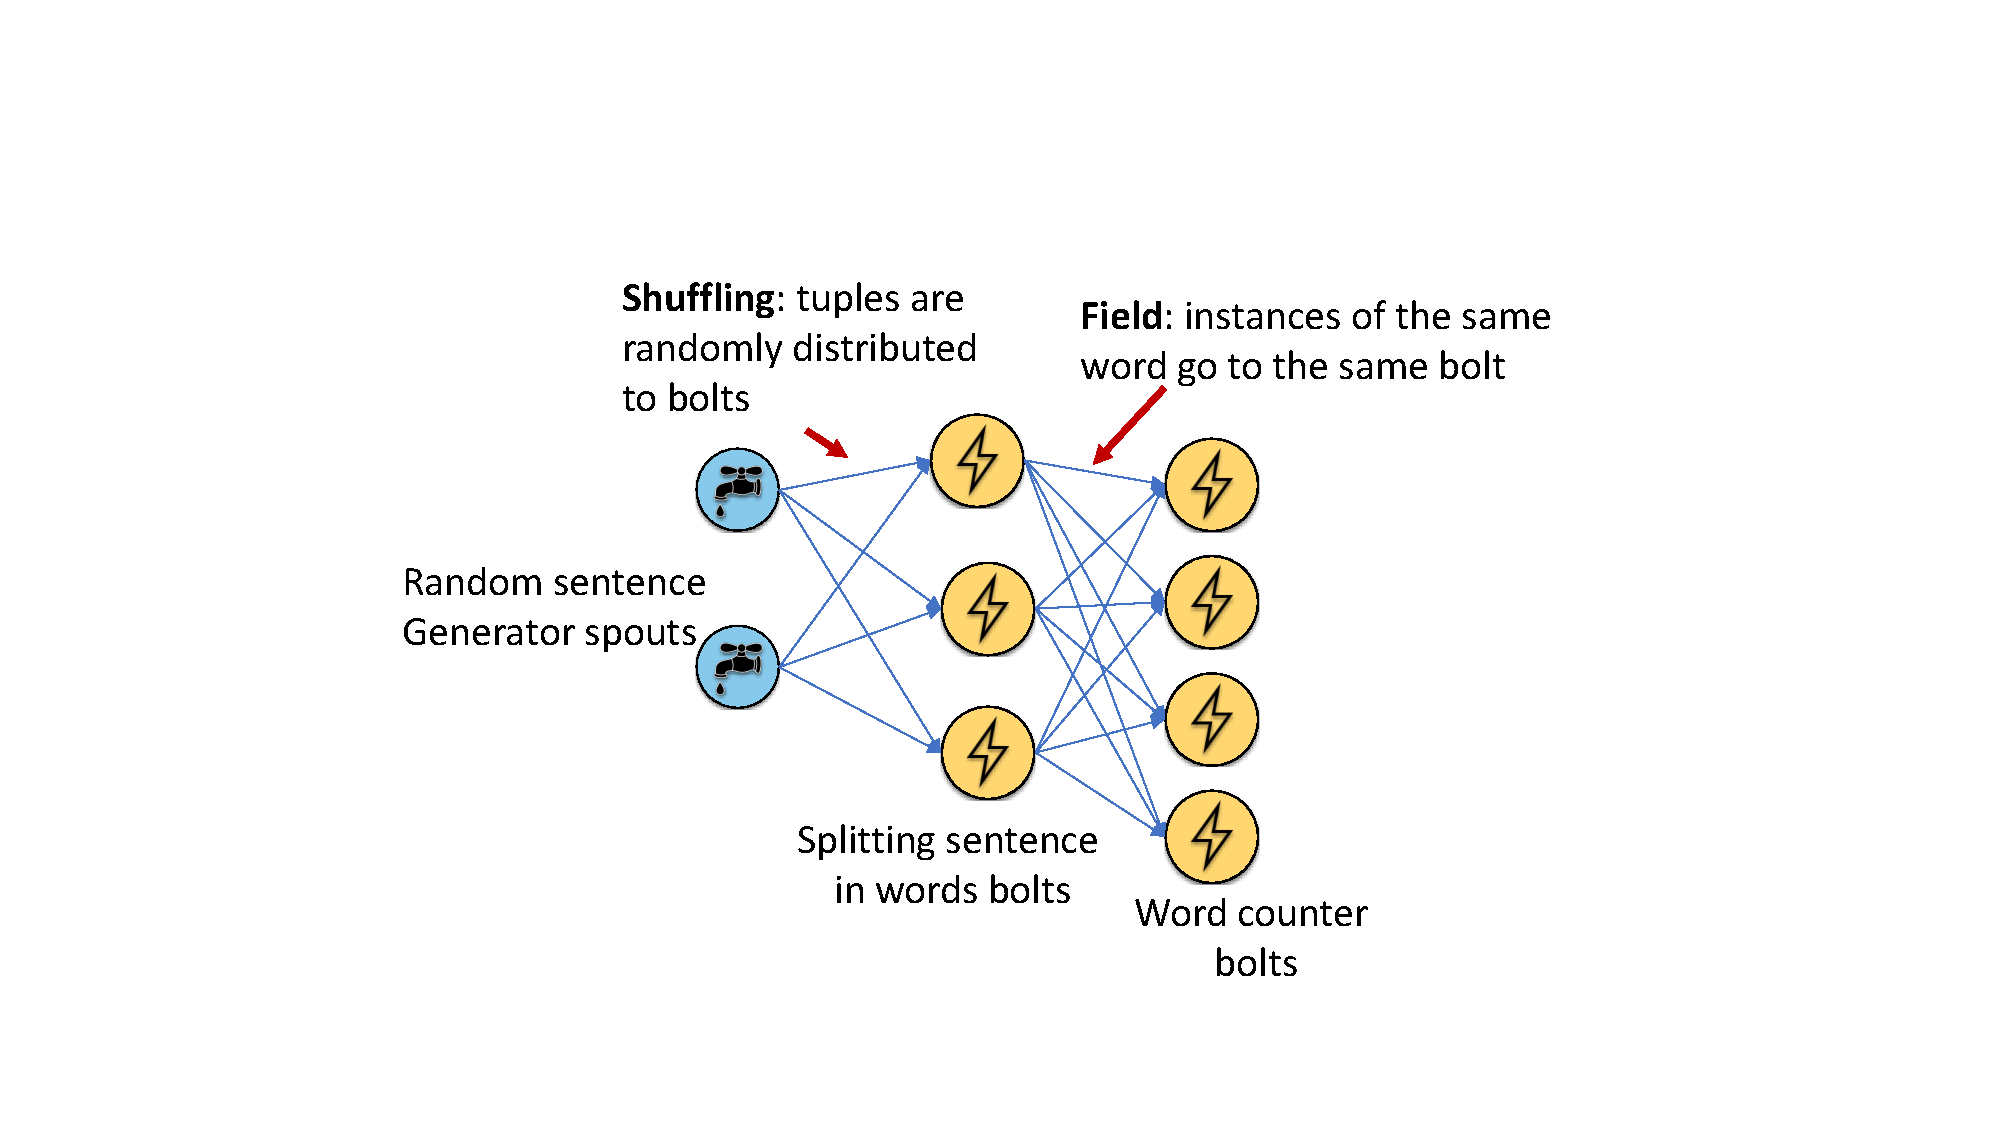
\includegraphics[width=\textwidth]{img/apache-storm.pdf}
    \end{center}
\end{examplebox}